
\section{The Tableau}\label{sec:tableau}
%
%
%We decide satisfiability of an input formula $\varphi$ by a depth-first, on-the-fly construction that
%builds a graph of symbolic nodes and searches it for a \emph{successful marking}. A node carries the
%formulas to be realised at a configuration, and zones represent clock valuations symbolically. A
%time-bounded modality is never tested against a precomputed set of valuations: it is discharged by
%\emph{pursuing} it, so that the search itself produces the witness. We fix nodes and realisability
%(\S\ref{ss:nodes}), give the rules (\S\ref{ss:rules}), define acceptance and its test
%(\S\ref{ss:loop}), and close with two examples (\S\ref{ss:ex}).
%
We decide satisfiability of $\varphi$ by an on-the-fly, symbolic tableau construction.
%
%A time-bounded modality is never tested against a precomputed set of valuations but discharged by
%\emph{pursuing} it, so that the search itself produces the witness. 
%
We fix nodes and realisability
(\S\ref{ss:nodes}), give the rules (\S\ref{ss:rules}), define acceptance (\S\ref{ss:loop}), and
close with two examples (\S\ref{ss:ex}).

\subsection{Nodes and Realisability}\label{ss:nodes}


A {node} is a tuple $N=\tup{\Gamma}{\Ctx}{Z}{\obligations}{\Deadline}$, where $\Gamma$ is the set of
goal formulas to be satisfied (write $\Gamma_{\mathsf{prop}}=\Gamma\cap\big(\mathcal P\cup\{\neg p\mid p\in\mathcal P\}\big)$ for the propositional part); $\Ctx$ the {context} of universal formulas that must
hold at every successor; $Z$ the set of clock valuations for this node, represented as a canonical zone; $\obligations$ the {clock map}, which allocates to every active timed modality $\mu$ a dedicated formula-clock $x_\mu$ so its window (i.e. its interval \kI) can be measured from the configuration that demanded it; and $\Deadline$ is a set of deadlines
$(x_\mu,\sup\kI)$, each with a strictness flag, and $\Inv(N)=\bigwedge_{(x_\mu,b)\in \Deadline}x_\mu\le b$
its induced invariant. Besides these five components a node records the clocks reset by the rule
that produced it and, if that rule was a stop branch, the modality it discharged; a rule sets both
from the branch it takes, and we leave them implicit in the displays below.

%%%%%%%%% DEAD TEXT %%%%%%%%
% $\equiv$ is defined again below, after realisability, and closedness both below
% and in \S\ref{ss:loop}.
%Two nodes are
%\emph{equivalent}, written $N\equiv N'$, when they agree in $\Gamma$, $\Ctx$, $\obligations$, $\Deadline$ and
%in these two records, and their zones agree modulo $\cong_M$. A node is \emph{closed} when
%$\Gamma_{\mathsf{prop}}$ contains a complementary pair $p,\neg p$ or its zone is empty. Closed
%nodes have no children.
%%%%%%%%% DEAD TEXT %%%%%%%%

%A deadline is added when \ruleref{Cov} launches the pursuit of a
%universal until and removed when the $(\text{stop})$ branch of \ruleref{Uunf} discharges it;
%no other rule writes $\Deadline$.
%
%; and $\eventualities$ the postponed eventualities used for loopacceptance. 


%Write $\Gamma_{\mathsf{prop}}=\Gamma\cap\big(\mathcal P\cup\{\neg p\mid p\in\mathcal P\}\big)$ for the {propositional part} of $\Gamma$, the atomic literals it asserts. A node is {closed} if $\Gamma_{\mathsf{prop}}$ is propositionally inconsistent, i.e., it contains a complementary pair $p,\neg p$ (equivalently $\bot\in\Gamma$), or its zone is empty, $Z=\emptyset$; it is {saturated} when no expansion rule applies.



%\noindent
%We write
%$\Gamma_{\mathsf{prop}}=\Gamma\cap\big(\mathcal P\cup\{\neg p\mid p\in\mathcal P\}\big)$ for the
%\emph{propositional part} of $\Gamma$, the atomic literals it asserts. 

%%%%%%%%% DEAD TEXT %%%%%%%%
% A path is defined again in \S\ref{ss:loop}, where the tableau graph is introduced
% and paths are first used.
%We call a sequence of nodes $N_0,N_1,\dots$ a \emph{path} if each $N_{i+1}$ is a child of $N_i$.
%%%%%%%%% DEAD TEXT %%%%%%%%

%Write
%\[
%  \Inv(N)\hspace{-0.1cm}=\hspace{-0.1cm}\bigwedge\big\{x_\mu\le\sup\kI \big| \mu=\mathrm{A}(\varphi\mathbf{U}_\kI\psi)
%  \text{ under pursuit at } N \big\} \quad (<\text{ if } \sup\kI\notin\kI)
%\]
%for the node's {invariant}. Both $x_\mu$ and the bound are read off the node: the clock
%from $\obligations$, the interval from $\mu$ itself.
%
%$\clocks(\obligations)$
A node is \emph{closed} if its zone is empty, $Z=\emptyset$, since it then has no valuations to
realise, or if $\bot\in\Gamma_{\mathsf{prop}}$. It is
\emph{saturated} when no saturation or cover rule applies; only saturated nodes generate successors.
It is \emph{realisable} if there is a non-blocking TTS $\mathcal T$ induced by a TA, a location $s$ with
$L(s)\supseteq\Gamma_{\mathsf{prop}}$ and $\Inv(s)=\Inv(N)$, and an interpretation of the
formula-clocks in \obligations, such that for every $\nu \in Z$ the configuration $(s,\nu)$  $\mathcal T,(s,\nu)\models\textstyle\bigwedge\Gamma\ \wedge\ \bigwedge\Ctx$. 
Realisability is {monotone under narrowing}: if $\tup{\Gamma}{\Ctx}{Z}{\obligations}{\Deadline}$ is realisable and
$\emptyset\neq Z'\subseteq Z$, then so is $\tup{\Gamma}{\Ctx}{Z'}{\obligations}{\Deadline}$.


%Two consequences of Definition~\ref{def:realisable} shape the calculus. First, the quantification over $Z$ is \emph{universal}: this is precisely what lets a single node discharge a demand re-imposed by a persistent context at a continuum of onsets. Second, realisability is \emph{monotone under narrowing}.

%\begin{lemma}[Narrowing]\label{lem:narrowing}
%If $\tup{\Gamma}{\Ctx}{Z}{\obligations}$ is realisable and
%$\emptyset\neq Z'\subseteq Z$, then $\tup{\Gamma}{\Ctx}{Z'}{\obligations}$ is realisable.
%\end{lemma}
%\begin{proof}
%Immediate: the condition of Definition~\ref{def:realisable} is universally quantified over the zone, and
%$Z'$ is a non-empty subset of $Z$.
%\end{proof}
%
%Lemma~\ref{lem:narrowing} is what licenses the refinement rule \ruleref{Covstar} to be a disjunctive
%choice rather than a case analysis: a node is free to commit to a tighter entry constraint. For this to
%be sound at the level of the extracted automaton, the narrowing must happen \emph{before} the node's
%outgoing steps are fixed; this is guaranteed by the discipline of \S\ref{ss:rules}, where a node is
%saturated and covered to exhaustion before any successor is generated, so the guards of its delays and
%edges are read off the narrowed zone.

%\noindent

Two nodes $N_1$ and $N_2$ are \emph{equivalent}, written $N_1\equiv N_2$, when they agree in $\Gamma$, $\Ctx$, $\obligations$, $\Deadline$, in the
clocks reset by the rule that produced them and in the modality that rule discharged, and their
zones agree modulo $\cong_M$.


An \emph{OR} (disjunctive, $\ORn$) node is realisable if
\emph{some} child is; an \emph{AND} (conjunctive, $\ANDn$) node requires \emph{all} its children. Some
rules are deterministic ($\DETn$): a single child, replacing the node.  We write $kind(N)\in\{\DETn,\ORn,\ANDn\}$.





%Table~\ref{tab:rulekinds} fixes the kind of every rule; the marginal marker on each rule below repeats it.

%\begin{table}[t]
%\centering
%\caption{Every rule and its branching kind. $\DETn$ = single child, $\ORn$ = OR-node,
%$\ANDn$ = AND-node.}\label{tab:rulekinds}
%\begin{tabular}{llll}
%\hline
%Group & Rule & Kind & Children \\
%\hline
%Saturation & $(\wedge)$, \ruleref{AX} & $\DETn$ & $1$ \\
%Saturation & $(\vee)$ & $\ORn$ & $2$ \\
%Cover & \ruleref{Cov} & $\ANDn$ & $2$ (discharge, launch) \\
%Cover & \ruleref{Covstar} & $\ORn$ & one per convex component \\
%Pursuit & \ruleref{Uunf} & $\ORn$ & $2$ (stop, go) \\
%Pursuit & \ruleref{Rsplit} & $\ANDn$ & $\le 3$ (before, in, after) \\
%Pursuit & \ruleref{Runf} & $\ORn$ & $2$ per part \\
%Successors & \ruleref{Delay} & $\ANDn$ & $2$ (open segment, boundary) \\
%Successors & \ruleref{EX} & $\ANDn$ & one per $\EX\psi\in\Gamma$, or stutter \\
%\hline
%\end{tabular}
%\end{table}
%
\noindent


%A \emph{marking} $\mathcal M$ selects one child at each OR-node and \emph{all} children at each
%AND-node; it is \emph{successful} if it contains no closed node and every postponed eventuality is
%fulfilled on every infinite path, in the sense made effective by the loop condition of
%\S\ref{ss:loop}. 



%The tableau \emph{succeeds} on $\varphi$ if the root
%$\tup{\{\varphi\}}{\emptyset}{\Zuniv}{\emptyset}{\emptyset}$ admits a successful marking, where
%$\Zuniv$ is the universal zone over $\clockSet$.

\subsection{Rules}\label{ss:rules}
Rules come in four groups: \emph{saturation} decomposes goals, \emph{cover} discharges and
launches a timed modality, \emph{pursuit} unfolds a launched one step by step, and
\emph{successor generation} expands a saturated node.
%Each rule rewrites a node into its children, shown on the full tuple; a component reappears unchanged unless the rule modifies it.
%
%We consider four groups of rules: \emph{saturation} decomposes the goals in $\Gamma$, the \emph{cover} rule discharges a timed modality, the \emph{pursuit} rules unfold a launched modality one step at a time, and \emph{successor generation} expands a saturated node in time and across edges.
%%
%%Rules come in four groups: \emph{saturation}
%%decomposes the goals in $\Gamma$, the \emph{cover} rule discharges a timed modality, the
%\emph{pursuit} rules unfold a launched modality one step at a time, and \emph{successor
%generation} expands a saturated node in time and across edges.
%
\vspace{-0.1cm}
\paragraph{Saturation.}
Conjunction \ruleref{Conj} is deterministic, disjunction \ruleref{Disj} branches, and \ruleref{AX} handles a universal marker by moving its argument into the context. %There is no saturation rule for $\EX$: ``some successor satisfies
%$\psi$'' cannot be settled before successors exist, so $\EX\psi$ waits in $\Gamma$ and is discharged by
%\ruleref{EX}.
\vspace{-0.1cm}
\[
\footnotesize
\ \frac{\tup{\Gamma\cup\{\varphi\land\psi\}}{\Ctx}{Z}{\obligations}{\Deadline}}
{\tup{\Gamma\cup\{\varphi,\psi\}}{\Ctx}{Z}{\obligations}{\Deadline}}\quad
\shortstack{\ruleanchor{Conj}\\\DETn}
\qquad
\ \frac{\tup{\Gamma\cup\{\AX\varphi\}}{\Ctx}{Z}{\obligations}{\Deadline}}
{\tup{\Gamma}{\Ctx\cup\{\varphi\}}{Z}{\obligations}{\Deadline}}\quad
\shortstack{\ruleanchor{AX}\\ \DETn}
\]\vspace{-0.2cm}
\[
\footnotesize
\frac{\tup{\Gamma\cup\{\varphi\lor\psi\}}{\Ctx}{Z}{\obligations}{\Deadline}}
{
\begin{array}{ll}
\tup{\Gamma\cup\{\varphi\}}{\Ctx}{Z}{\obligations}{\Deadline}\\
  \tup{\Gamma\cup\{\psi\}}{\Ctx}{Z}{\obligations}{\Deadline}
\end{array}
}
%
%\ \frac{\tup{\Gamma\cup\{\varphi\lor\psi\}}{\Ctx}{Z}{\obligations}{\Deadline}}
%{\tup{\Gamma\cup\{\varphi\}}{\Ctx}{Z}{\obligations}{\Deadline}\quad\big|\quad
%\tup{\Gamma\cup\{\psi\}}{\Ctx}{Z}{\obligations}{\Deadline}}
\quad
\shortstack{\ruleanchor{Disj}\\\ORn
}
\]

\paragraph{Pursuing time modalities.}

When $\Gamma$ contains a timed modality $\mu=\mathrm{Q}(\varphi\circ_\kI\psi)$, with
$\mathrm{Q}\in\{\mathrm{E},\mathrm{A}\}$ and $\circ\in\{\mathbf{U},\mathbf{R}\}$, we say the node
\emph{demands} $\mu$, and $\mu$ must hold at every valuation of the node's zone. To fulfil the demand the rule produces a \ruleref{discharge} child, which drops $\mu$ from
$\Gamma$ and lets the node continue with its remaining goals, and a \ruleref{launch} child, which
starts a \emph{pursuit} of $\mu$, written $\mu^\bullet$, i.e., a branch that unfolds $\mu$ step by
step in search of a witness. The launch introduces a fresh formula-clock $x_\mu$ and resets it
here, so that $\kI$ is measured from this configuration.

\vspace{-0.3cm}
\[
\footnotesize
\frac{\tup{\Gamma\cup\{\mu\}}{\Ctx}{Z}{\obligations}{\Deadline}}
{\begin{array}{ll}
\tup{\Gamma}{\Ctx}{Z}{\obligations}{\Deadline} & \ruleanchor{discharge}\\[3pt]
\tup{\Gamma\cup\{\mu^\bullet\}}{\Ctx}{\rst{Z}{x_\mu}}{\obligations[\mu\mapsto x_\mu]}{\Deadline\cup \Deadline_\mu}
 & \ruleanchor{launch}
\end{array}}
\raisebox{-4ex}{
  \shortstack{
    $\obligations(\mu)$ undefined, or\\
    $\sup\kI<\infty$ and $\mu$ not\\
    a universal until}
}
\shortstack{\ruleanchor{Cov}\\\ANDn}
\]


%The rule is conjunctive because its children carry different work for one and the same
%configuration: the launches are what \emph{establish} $\mu$, one onset each, and the discharge is
%what lets the rest of $\Gamma$ be established alongside them. They are not alternatives, and none
%may be dropped. In particular the cross-product of the branches over several demands is what
%forces every demand of a node into a common leaf, where a contradiction between them closes it.
%
A deadline $\Deadline_\mu=\{(x_\mu,\sup\kI)\}$ is applied iff $\mu$ is a universal until, with
$\Deadline_\mu=\emptyset$ otherwise. Only such a modality needs one, as it obliges \emph{every} run to
satisfy $\psi$ within $\kI$ and time must be forced forward or a run could idle past the window with
the eventuality unmet. An existential until is discharged by a single witnessing run, and a release,
of either quantifier, is discharged by lapsing past the window rather than by acting within it.

%
%The side condition fires \ruleref{Cov} on a modality not yet under pursuit, and on one already
%pursued when its window is finite and it is not a universal until.
%

%A window with
%$\sup\kI=\infty$ leaves no bound to carry either way, and there the eventuality is forced instead by
%the acceptance condition on markings (\S\ref{ss:loop}).
%
%What that sharing costs is settledwhere the pursuit succeeds.

%Because the demand is discharged by construction, the calculus never has to narrow a node to the
%part of its zone on which $\mu$ happens to hold. Narrowing survives
%only where a rule genuinely partitions the zone, in \ruleref{Rsplit} and \ruleref{Delay} below, and
%it is there that monotonicity of realisability under narrowing is used.

\paragraph{Pursuing an Until.}





Consider an until modality $\mu=\mathrm{Q}(\varphi\mathbf{U}_\kI\psi)$, writing
$a=\inf\kI$ and $b=\sup\kI$. An ordinary pursuit $\mu^\bullet$ unfolds by \ruleref{Uunf}: either
$\psi$ holds now, inside the window, or $\varphi$ holds now and the pursuit passes to the
successors.
%
%
%Its unfolding is a disjunction: either $\psi$ holds now and the
%eventuality is met, which is the \ruleref{Ustop} branch, or $\varphi$ holds now and the pursuit is
%deferred to the successors, which is \ruleref{Ugo}. We call a pursuit \emph{persistent} once
%\ruleref{Carry} has folded a re-demand into it; for such a pursuit the stop branch takes a different
%form. 
\vspace{-0.1cm}
\[
\footnotesize
\frac{\tup{\Gamma\cup\{\mu^\bullet\}}{\Ctx}{Z}{\obligations}{\Deadline}}
{\begin{array}{ll}
\tup{\Gamma\cup\{\psi\}}{\Ctx}{Z\cap(x_\mu\in\kI)}{\obligations}{\Deadline\setminus\{(x_\mu,b)\}}
  & \ruleanchor{Ustop}\\[4pt]
\left\{
\begin{array}{ll}
\tup{\Gamma\cup\{\varphi,\EX\mu^\bullet\}}{\Ctx}{Z}{\obligations}{\Deadline}
  & \text{if } \mathrm{Q}=\mathrm{E},\\[3pt]
\tup{\Gamma\cup\{\varphi\}}{\Ctx\cup\{\AX\mu^\bullet\}}{Z}{\obligations}{\Deadline}
  & \text{if } \mathrm{Q}=\mathrm{A},
\end{array}
\right.
& \ruleanchor{Ugo}
\end{array}}
\shortstack{
$\mu=\mathrm{Q}(\varphi\mathbf{U}_\kI\psi)$}
\shortstack{\ruleanchor{Uunf}\\\ORn}
\]
\ruleref{Ugo} defers the pursuit to the successors, where $x_\mu$ keeps running and the window
stays open; for $\mathrm{Q}=\mathrm{E}$ a single witnessing run suffices, so the residual travels
as a goal to one successor, and for $\mathrm{Q}=\mathrm{A}$ every run must comply, so it travels
as context to all of them. \ruleref{Ustop} ends the pursuit: $\mu^\bullet$ is dropped from
$\Gamma$ and its deadline removed from $\Deadline$, the single onset it was launched for having
been answered.

Pursuit must end when the window closes, i.e., $x_\mu\in\kI$ fails. The rule \ruleref{Umiss} empties the zone and closes the node, which is then no longer realisable.
%
%Deferral ends with the window. The witness needs $x_\mu\in\kI$ and the clock only grows, so a
%zone lying wholly beyond a finite $b$ holds no moment for it; \ruleref{Umiss} empties the zone,
%and the node is closed.
\vspace{-0.2cm}
\[
\footnotesize
\frac{\tup{\Gamma\cup\{\mu^\bullet\}}{\Ctx}{Z}{\obligations}{\Deadline}}
     {\tup{\Gamma\cup\{\mu^\bullet\}}{\Ctx}{\emptyset}{\obligations}{\Deadline}}
\quad
\begin{array}{l}
%Z\cap(x_\mu\le b)=\emptyset,\\ b<\infty
x_\mu\not\in\kI, \\ b<\infty
\end{array}
\shortstack{\ruleanchor{Umiss}\\\DETn}
\]
For a universal until the deadline in
$\Deadline$ empties the zone first and the rule never fires.

%; for an existential until it settles
%the eventuality, \ruleref{Ugo} alone being available at every step. 
%%The rule carries no
%invariant: an existential demand is served by a single run, and an invariant binds them all.
%
\begin{figure}[t]
\centering
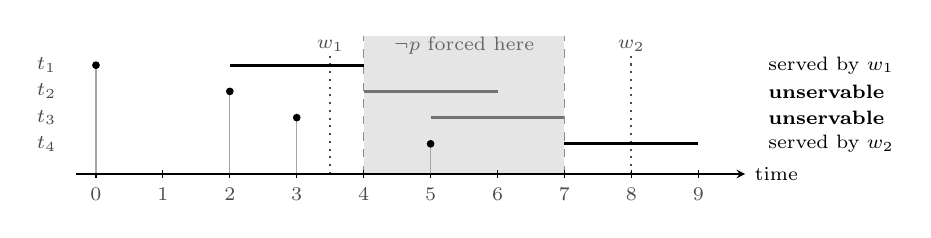
\begin{tikzpicture}[x=8.5mm,y=3.33mm,font=\scriptsize,>=stealth]

% band where p is forbidden
\fill[black!10] (4,-0.75) rectangle (7,4.5);
\draw[black!45,dashed] (4,-0.75) -- (4,4.5);
\draw[black!45,dashed] (7,-0.75) -- (7,4.5);
\node[black!60] at (5.5,4.15) {$\lnot p$ forced here};

% candidate times for p
\draw[black!70,dotted,thick] (3.5,-0.75) -- (3.5,3.9);
\node[black!70] at (3.5,4.15) {$w_1$};
\draw[black!70,dotted,thick] (8,-0.75) -- (8,3.9);
\node[black!70] at (8,4.15) {$w_2$};

% time axis
\draw[->] (-0.3,-0.75) -- (9.7,-0.75) node[right] {time};
\foreach \t in {0,1,2,3,4,5,6,7,8,9}
  \draw (\t,-0.9) -- (\t,-0.6) node[below=3pt,black!70] {$\t$};

% onset marks, named on the left
\foreach \o/\r/\lab in {0/3.4/{$t_1$}, 2/2.4/{$t_2$}, 3/1.4/{$t_3$}, 5/0.4/{$t_4$}} {
  \node[anchor=east,black!70] at (-0.45,\r) {\lab};
  \draw[black!35] (\o,\r) -- (\o,-0.7);
  \fill (\o,\r) circle (1.4pt);
}
% windows [t_i+2, t_i+4]
\draw[very thick] (2,3.4) -- (4,3.4);
\draw[very thick,black!55] (4,2.4) -- (6,2.4);
\draw[very thick,black!55] (5,1.4) -- (7,1.4);
\draw[very thick] (7,0.4) -- (9,0.4);

\node[anchor=west] at (9.9,3.4) {served by $w_1$};
\node[anchor=west] at (9.9,2.4) {\textbf{unservable}};
\node[anchor=west] at (9.9,1.4) {\textbf{unservable}};
\node[anchor=west] at (9.9,0.4) {served by $w_2$};

\end{tikzpicture}
\caption{The formula $\mathrm{AG}\,\mathrm{EF}_{[2,4]}\,p\wedge\mathrm{AG}_{[4,7]}\lnot p$ (\UNSAT). The bar at
$t_i$ is that onset's window $[t_i+2,t_i+4]$, and a $p$ at $w$ serves the onsets whose bar contains
it. The pursuit launched at $t_1$ stops at $w_1$ and serves no later onset.}\label{fig:onsets}
\end{figure}


As shown in Fig.~\ref{fig:onsets}, a demand can be potentially requested by a continuum of onsets. We handle it symbolically, according to whether $\sup I < \infty$ or not. 

\noindent
For $\sup I=\infty$, the new onset is absorbed into the running one: \ruleref{Absorb} drops
$\mu$ from $\Gamma$, so it is not demanded again, and keeps the previous pursuit alive. A new
one is launched only when the previous pursuit stops, so a run carries a stream of witnesses,
and every onset here asks only for a $\psi$ at some later point, which the stream supplies. 

\noindent
For $\sup I<\infty$, some onsets can not be absorbed, as shown in Fig.~\ref{fig:onsets}. In this case, we distinguish between the existential until, which is simply pursued by a new \ruleref{Cov}, and a universal until, which is \emph{carried}. Every run must comply with the demand, so one pursuit that witnesses at least every $b-a$ covers every onset and it turns \emph{persistent}, written $\mu^{\ast}$, which is unfolded by \ruleref{Uunfcarry}. 
\vspace{-0.2cm}
\[
\footnotesize
\frac{\tup{\Gamma\cup\{\mu,\mu^\bullet\}}{\Ctx}{Z}{\obligations}{\Deadline}}
     {\tup{\Gamma\cup\{\mu^{\ast}\}}{\Ctx}{Z}{\obligations}{\Deadline}}
  \hspace{-0.25cm}
\shortstack{
%$\mu=\mathrm{A}(\varphi\mathbf{U}_\kI\psi),$\\
$\mu$ universal \\ until,\\
$b<\infty$
}
\hspace{-0.33cm}
\shortstack{\ruleanchor{Carry}\\\DETn}
\hspace{0.2cm}
\footnotesize
\frac{\tup{\Gamma\cup\{\mu,\mu^{\dagger}\}}{\Ctx}{Z}{\obligations}{\Deadline}}
     {\tup{\Gamma\cup\{\mu^{\dagger}\}}{\Ctx}{Z}{\obligations}{\Deadline}}
\hspace{-0.37cm}
\raisebox{0ex}{
\shortstack{
$\mu^{\dagger}\in\{\mu^{\bullet},\mu^{\ast}\},$\\
$b=\infty\ \text{or}$\\
$ \mu^{\dagger}=\mu^{\ast}$
}
}
\hspace{-0.4cm}
\shortstack{\ruleanchor{Absorb}\\\DETn}
\]
\vspace{-0.35cm}
\[
\footnotesize
\frac{\tup{\Gamma\cup\{\mu^{\ast}\}}{\Ctx}{Z}{\obligations}{\Deadline}}
{\begin{array}{ll}
\tup{\Gamma\cup\{\psi,\mu^{\ast}\}}{\Ctx}{\rst{Z\cap(x_\mu\in\kIrec)}{x_\mu}}{\obligations}
{\Deadline[x_\mu\mapsto b-a]}
  & \ruleanchor{Ustopcarry}\\[4pt]
\tup{\Gamma\cup\{\varphi\}}{\Ctx\cup\{\AX\mu^{\ast}\}}{Z}{\obligations}{\Deadline}
  & \ruleanchor{Ugocarry}
\end{array}}
\hspace{-0.1cm}
\raisebox{-3ex}{
\shortstack{
$ b<\infty$\\
$\mu=\mathrm{A}(\varphi\mathbf{U}_\kI\psi)$
}
}
\hspace{-0.5cm}
\shortstack{\ruleanchor{Uunfcarry}\\\ORn}
\]
\ruleref{Ustopcarry} keeps the pursuit alive. A persistent pursuit answers every onset carried
into it, and the context keeps raising more, so $\mu^{\ast}$ stays and its clock restarts:
$x_\mu$ is re-zeroed, measuring from this occurrence of $\psi$, and its deadline is set to
$b-a$. That bound is the length of the window. A time $w$ at which $\psi$ holds answers exactly the
onsets in $[w-b,w-a]$, so two consecutive such times leave no onset unanswered precisely when
they lie within $b-a$ of each other. The guard follows the same reading: $\kIrec$ is \kI\ at the
first witness, where $x_\mu$ still measures from the onset that launched the pursuit, and $[0,b-a]$
at every later one, where it measures from the preceding witness. 

%Reading \kI\ throughout would ask
%consecutive witnesses to be at least $a$ apart while $\Deadline$ caps them at $b-a$, and for
%$2a>b$ no witness could follow the first.

%Take $\tAU{\top}{q}{[1,4]}$ demanded at every configuration. Witnesses four apart, at $0,4,8,\dots$,
%will not do: the onset at $3.5$ needs a $q$ in $[4.5,7.5]$, and the witness at $4$ is too early while
%the one at $8$ is too late. Witnesses three apart, at $0,3,6,\dots$, do: every window $[t+1,t+4]$ has
%length three, and points spaced three apart meet every interval of that length. The lower endpoint
%only shifts the window along the timeline; its length, $b-a$, is what fixes the rate. Read from the
%witness rather than the window, the same bound says that the oldest onset a witness at $w$ leaves
%unanswered lies just past $w-a$, has already waited $a$, and so runs out at $w+(b-a)$.
%%
%Where $b=\infty$ the bound is vacuous, every onset up to $w-a$ being answered at $w$, and all that
%survives of the requirement is that such times keep occurring. That is an eventuality with no
%deadline, which no invariant can bound and the acceptance condition on markings
%(\S\ref{ss:loop}) carries instead, so \ruleref{Carry} asks for a finite window.
%
%

%%%% Maybe adding it in the loop part later
%For $\mathrm{Q}=\mathrm{E}$
%no cap is needed, because $\mu$ was placed in $\eventualities$ at launch and a run that defers forever
%yields a non-fulfilling loop, rejected by \S\ref{ss:loop}; adding the cap there would only prune, never
%change the verdict.
%

\paragraph{Pursuing a Release.}
Consider now a release modality $\mu=\mathrm{Q}(\varphi\mathbf{R}_\kI\psi)$. The semantics of release imposes that $\psi$ must hold at every point in the window, unless $\varphi$ releases it. We handle the pursuit of a release in two stages. First, we partition the zone according to the position of $x_\mu$ relative to $\kI$, and then we pursue each part separately. We write $\ZltI = Z\cap(x_\mu<\inf\kI$ or $ x_\mu=\inf\kI\notin\kI)$, $\ZinI = Z\cap(x_\mu\in\kI)$ and $\ZgtI = Z\cap(x_\mu>\sup\kI$ or $ x_\mu=\sup\kI\notin\kI)$ for the three parts of the partition,
%
%
%\begin{align*}
%    \ZltI = Z&\cap(x_\mu<\inf\kI\ \text{or}\ x_\mu=\inf\kI\notin\kI),\quad \ZinI = Z\cap(x_\mu\in\kI),\quad\\
%    &\ZgtI = Z\cap(x_\mu>\sup\kI\ \text{or}\ x_\mu=\sup\kI\notin\kI),
%\end{align*}
%
so that the strictness of the interval endpoints is carried by the DBM bounds and the three parts are a partition of $Z$. Empty parts are dropped. Accordingly, the unfolding of a release produces up to three children, one for each part of the partition. The first two are pursued, while the last is lapsed and drops $\mu^\bullet$.
\vspace{-0.2cm}
\[
\footnotesize
\frac{\tup{\Gamma\cup\{\mu^\bullet\}}{\Ctx}{Z}{\obligations}{\Deadline}}
{\begin{array}{lll}
\tup{\Gamma\cup\{\mu^\bullet\}}{\Ctx}{\ZltI}{\obligations}{\Deadline} & \ruleanchor{Rsplitbefore}\\[2pt]
\tup{\Gamma\cup\{\mu^\bullet\}}{\Ctx}{\ZinI}{\obligations}{\Deadline} & \ruleanchor{Rsplitin}\\[2pt]
\tup{\Gamma}{\Ctx}{\ZgtI}{\obligations}{\Deadline} & \ruleanchor{Rsplitafter}
\end{array}}
\quad \mu=\mathrm{Q}(\varphi\mathbf{R}_\kI\psi)
\shortstack{\ruleanchor{Rsplit}\\\ANDn}
\]

The \ruleref{Rsplitbefore} and \ruleref{Rsplitin} parts are pursued by the following rule, which, similarly to \ruleref{Uunf} is a disjunction between two cases: either $\varphi$ is released, or the pursuit continues. %The \ruleref{Rsplitafter} part is lapsed and drops $\mu^\bullet$.
%Within the before and in parts the pursuit then either discharges through $\varphi$ or continues; this is a choice, hence an OR-node.
\vspace{-0.2cm}
\[
\footnotesize
\frac{\tup{\Gamma\cup\{\mu^\bullet\}}{\Ctx}{Z}{\obligations}{\Deadline}}
{\begin{array}{ll}
\tup{\Gamma\cup\Theta\cup\{\varphi\}}{\Ctx}{Z}{\obligations}{\Deadline} & \ruleanchor{Rstop}\\[3pt]
\left\{
\begin{array}{ll}
\tup{\Gamma\cup\Theta\cup\{\EX\mu^\bullet\}}{\Ctx}{Z}{\obligations}{\Deadline} & \text{if } \mathrm{Q}=\mathrm{E},\\[2pt]
\tup{\Gamma\cup\Theta}{\Ctx\cup\{\AX\mu^\bullet\}}{Z}{\obligations}{\Deadline} & \text{if } \mathrm{Q}=\mathrm{A},
\end{array}
\right.
& \ruleanchor{Rgo}
\end{array}}
\raisebox{-2ex}{\shortstack{$Z\subseteq\ZltI$ and $\Theta=\emptyset$,\\
or $Z\subseteq\ZinI$ and $\Theta=\{\psi\}$}}
\shortstack{\ruleanchor{Runf}\\\ORn}
\]



%\ruleref{Rstop} settles the demand at once and drops $\mu^\bullet$, while \ruleref{Rgo} defers it
%as \ruleref{Ugo} does.



\paragraph{Successor generation.}
A saturated and covered node is expanded by two successor rules.%, one elapsing time and one taking discrete steps.
%\emph{Both are AND-rules}: a model must admit the passage of time \emph{and} supply every demanded edge.
%The choice between waiting and moving is not made here --- it is made by the \ruleref{Ustop}/\ruleref{Ugo} branching of \ruleref{Uunf} and the corresponding 
%\ruleref{Runf_before}/\ruleref{Runf_in} branching of \ruleref{Runf}, which is where the existential content of the calculus lives.
\ruleref{Delay} advances the zone to the next integer hyperplane $x=b$ ($b\le M$) of an active bound,
and does so in two steps: $\Dopen Z$ is the time-successor of $Z$ strictly below the next
hyperplane, and $\Dbd Z$ is that hyperplane (equivalently $\uparrow Z$ when no hyperplane remains at or
below $M$). The hyperplanes of $x_\mu$ are the endpoints of $\kI$ together with their
\emph{shifts} $\inf\kI-\inf\kJ$ and $\sup\kI-\sup\kJ$ by the window \kJ\ of every other modality of
$\varphi$. The shifts are what keep onsets apart: a $\mu$ banning $\psi$ over $\kI$ leaves a demand
for $\psi$ over $\kJ$ unsatisfiable exactly at the onsets in $[\inf\kI-\inf\kJ,\sup\kI-\sup\kJ]$, and
splitting $x_\mu$ at the endpoints of \kI\ alone leaves that interval inside a cell that also holds
satisfiable onsets, whose witness then discharges the whole cell. There are two shifts per pair of
modalities and none depends on the magnitude of a constant, so the count of hyperplanes stays
quadratic in $|\varphi|$ and flat in $M$. %Both are computed under the node's invariant, which is where $\Inv(N)$ bounds the elapse:
\vspace{-0.2cm}
\[
\footnotesize
 \frac{\tup{\Gamma}{\Ctx}{Z}{\obligations}{\Deadline}}
{\begin{array}{ll}
\tup{\Gamma}{\Ctx}{\Dopen Z\cap\Inv(N)}{\obligations}{\Deadline} & \ruleanchor{openseg}\\[2pt]
\tup{\Gamma}{\Ctx}{\Dbd Z\cap\Inv(N)}{\obligations}{\Deadline} & \ruleanchor{boundary}
\end{array}}
\quad  \shortstack{$\Gamma$ \text{ saturated }\\ \text { and covered}}
\shortstack{\ruleanchor{Delay}\\ \ANDn }
\]

The two children carry the same demands and differ only in their zone, and that difference is
what a guard is tested against. Take a pursuit of $\mathrm{E}(p\mathbf{U}_{[1,2)}q)$ on the
zone $x_\mu\in(1,2)$, with $x_\mu=2$ the next hyperplane. On \ruleref{openseg} the
\ruleref{Ustop} guard $x_\mu\in[1,2)$ is non-empty, so $q$ may still be witnessed; on \ruleref{boundary} it is empty, the window having closed, and only \ruleref{Ugo} survives with an
eventuality that can no longer be met. A single zone spanning both would have to answer once
for two regions, and $[1,2)$ would become indistinguishable from $[1,2]$. Splitting keeps them
apart at no cost in the extracted automaton, where a chain of delay steps is one continuous
elapse within a single location.

%The goals are carried unchanged across a delay: a delay does not change location, and the pursuit residuals in $\Gamma$ are obligations of the run, not of a single configuration, so they must survive it.
%Saturation is re-run at each delay successor, since the narrowed zone may newly satisfy or falsify a guard.

\ruleref{EX} takes the discrete steps and discharges the existential markers, one child per demanded
$\EX\psi$, each carrying $\psi$ under the full context:
\vspace{-0.2cm}
\[
\footnotesize
\ \frac{\tup{\Gamma}{\Ctx}{Z}{\obligations}{\Deadline}}
{\big(\ \tup{\{\psi\}\cup\Ctx}{\Ctx}{Z}{\obligations}{\Deadline}\ \big)_{\EX\psi\in\Gamma}}
\quad  \shortstack{$\Gamma$ \text{ saturated }\\ \text { and covered}}
\shortstack{\ruleanchor{EX}\\ \ANDn }
\]
When no $\EX\psi\in\Gamma$, a single \emph{stutter} child
$\tup{\Ctx}{\Ctx}{Z}{\obligations}{\Deadline}$ keeps the run alive. Each child inherits $\Ctx$, allowing \ruleref{AX} to take effect, and it is why universal obligations constrain the whole
branching rather than one path. A pursuit's residual rides both kinds of successor: $\EX\mu^\bullet$ in $\Gamma$ reaches one, $\AX\mu^\bullet$ in $\Ctx$ reaches all. So $x_\mu$ advances by elapsing time as well as across edges.
A timed window is therefore entered by delay, its in-window stop taken at the first successor that
satisfies it; a pure-delay witness, i.e., waiting in one location until $x_\mu\in\kI$, then stopping, is a
chain of time-successors ending in a stop, the stutter step supplying a discrete anchor only when the
location must be left.

%% Proposed replacement for \subsection{Acceptance} in sec/section4_nosat.tex.
%% Keeps the label ss:loop and the labels M1, M2; adds def:children, def:graph.
%% 
% \rlink expands to bare math; \rl is the text-mode-safe form used below.
\newcommand{\rl}[1]{\ensuremath{\rlink{#1}}}

\subsection{Two Worked Runs of The Tableau}\label{ss:ex}


Consider the formula $\mathrm{AG}\,\mu\wedge\mathrm{AG}(q\rightarrow\sigma)$ with $\mu=\tAU{\top}{q}{[1,4]}$, that is $\mathrm{AF}_{[1,4]}q$, and 
$\sigma=\tAR{\bot}{\neg q}{(0,3]}$, that is $\mathrm{AG}_{(0,3]}(\lnot q)$. The first conjunct demands a $q$ within
$[1,4]$ of every configuration; the second forbids a $q$ for $3$ time units after each one. The left conjunct proceeds as a persistent demand. Its first demand launches $\mu^\bullet$ with $x$
reset and the deadline $x\le\sup\kI=4$; the next re-demand meets a live pursuit, so \ruleref{Carry}
folds it in and the pursuit becomes $\mu^{\ast}$. Meanwhile the right conjunct re-imposes its body
$\neg q\vee\sigma$ at every configuration, so $N_2$ carries both, and the disjunction is settled
before $\mu^{\ast}$ is unfolded.
\noindent
Take $\neg q$, at $N_3$. The pursuit can then neither take \ruleref{Ustopcarry} nor \ruleref{Ugocarry}: \ruleref{Ustopcarry} would assert
$q$ into a goal set already holding $\neg q$, and \ruleref{Ugocarry} can only defer, which past $x=4$
empties the zone against the deadline. Both children close.
\noindent
Take $\sigma$ instead. It is launched with its own clock $z$ reset, and \ruleref{Ustopcarry} asserts
$q$, re-zeroing $x$ and recapping it at $b-a=3$; this is $N_4$, where the two clocks begin to run
together, $x=z$. That is the contradiction. The carried deadline $x\le3$ says the next $q$ is due
within $3$, while $\sigma$ forbids $q$ for as long as $z\in(0,3]$. At $N_5$ the \ruleref{Ustopcarry} branch needs a
$q$ it cannot have, and \ruleref{Ugocarry} needs $x>3$, which the deadline denies. Both children close,
so $N_2$ closes and the formula is \UNSAT.


\begin{figure}[h]
\centering
\begin{subfigure}[b]{0.5\textwidth}\centering
\resizebox{0.8\linewidth}{!}{%
\begin{tikzpicture}[
  every node/.style={align=center, font=\scriptsize},
  level 1/.style={sibling distance=26mm, level distance=9mm},
  level 2/.style={sibling distance=30mm, level distance=11mm},
  level 3/.style={sibling distance=15mm, level distance=11mm},
  level 4/.style={sibling distance=15mm, level distance=11mm},
  edge from parent/.style={draw,-}
]
\node {$N_0:\{\mathrm{AG}\,\mu\wedge\mathrm{AG}(q\!\rightarrow\!\sigma)\}\ \ANDn$}
 child { node {$N_1:\{\,\}$\\ $\OPEN$}
   edge from parent node[left,font=\tiny,pos=.45]{\rl{discharge}} }
 child { node {$N_2:\{\mu^{\ast},\neg q\vee\sigma\},\ x{:=}0$\\ $\Deadline{=}\{x\le 4\}\ \ORn$}
   child { node {$N_3:\{\neg q,\mu^{\ast}\}\ \ORn$}
     child { node {$\CLOSED$\\ $q\wedge\neg q$}
       edge from parent node[left,font=\tiny,pos=.45]{\rl{Ustopcarry}} }
     child { node {$\CLOSED$\\ $\rl{Ugocarry}$\\ needs $x>4$}
       edge from parent node[right,font=\tiny,pos=.45]{\rl{Ugocarry}} }
     edge from parent node[left,font=\tiny,pos=.45]{$\neg q$} }
  child { node {$N_4:\{q,\mu^{\ast},\sigma^\bullet\}$\\ $x{:=}0,\ z{:=}0,\ \Deadline{=}\{x\le3\}$}
     child { node {$N_5:\{\neg q,\mu^{\ast},\sigma^\bullet\}$\\ $x{=}z\in(0,3]\ \ORn$}
       child { node {$\CLOSED$\\ \rl{Ustopcarry} \\needs $q$}
         edge from parent node[left,font=\tiny,pos=.45]{\rl{Ustopcarry}} }
       child { node {$\CLOSED$\\ \rl{Ugocarry} \\needs $x>3$}
         edge from parent node[right,font=\tiny,pos=.45]{\rl{Ugocarry}} }
       edge from parent node[right,font=\tiny,pos=.45]{\rl{Delay}, \rl{EX}} }
     edge from parent node[right,font=\tiny,pos=.4]{$\sigma$; \rl{launch}, \rl{Ustopcarry}} }
   edge from parent node[right,font=\tiny,pos=.45]{$(\wedge)$, \rl{launch}, \rl{Carry}} };
\end{tikzpicture}}
\subcaption{$\mathrm{AG}(\mathrm{AF}_{[1,4]} q)\wedge\mathrm{AG}(q \rightarrow
\mathrm{AG}_{(0,3]}(\lnot q))$.}
\label{fig:ex-roll}
\end{subfigure}
\hfill
\begin{subfigure}[b]{0.48\textwidth}\centering
\resizebox{0.9\linewidth}{!}{%
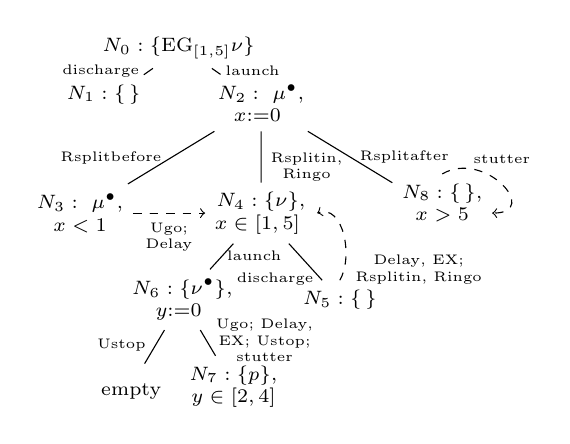
\begin{tikzpicture}[
  every node/.style={align=center, font=\scriptsize},
  level 1/.style={sibling distance=20mm, level distance=7mm},
  level 2/.style={sibling distance=23mm, level distance=14mm},
  level 3/.style={sibling distance=20mm, level distance=11mm},
  level 4/.style={sibling distance=13mm,level distance=11mm},
  edge from parent/.style={draw,-}
]
\node {$N_0:\{\mathrm{EG}_{[1,5]}\nu\}\ \ANDn$}
 child { node {$N_1:\{\,\}$\\ $\OPEN$}
   edge from parent node[left,font=\tiny,pos=.45]{\rl{discharge}} }
 child { node {$N_2:\ \mu^\bullet,$\\$x{:=}0\ \ANDn$}
   child { node (bef) {$N_3:\ \mu^\bullet,$\\$ x<1$}
    edge from parent node[left,font=\tiny,pos=.5]{\rl{Rsplitbefore}} }
   child { node (in) {$N_4:\{\nu\},$\\$ x\in[1,5]\ \ANDn$}
     child { node {$N_6:\{\nu^\bullet\},$\\$ y{:=}0\ \ORn$}
       child { node {$\CLOSED$\\ empty}
         edge from parent node[left,font=\tiny,pos=.45]{\rl{Ustop}} }
       child { node {$N_7:\{p\},$\\$ y\in[2,4]$}
         edge from parent node[right,font=\tiny,pos=.4]{\rl{Ugo}; \rl{Delay},\\ \rl{EX}; \rl{Ustop}; \\stutter} }
       edge from parent node[right,,xshift=-2pt,font=\tiny,pos=.45]{\rl{launch}} }
       child { node (disch) {$N_5:\{\,\}$}
       edge from parent node[left, yshift=-7pt,xshift=7pt,font=\tiny,pos=.45]{\rl{discharge}} }
     edge from parent node[right,font=\tiny,pos=.7]{\rl{Rsplitin},\\ \rl{Ringo}} }
   child { node (aft) {$N_8:\{\,\},$\\$ x>5$\\ $\OPEN$}
     edge from parent node[right,font=\tiny,pos=.5]{\rl{Rsplitafter}} }
   edge from parent node[right,font=\tiny,pos=.45]{\rl{launch}} };
\draw[->,dashed] (bef.east) to[out=0,in=180,looseness=.7]
  node[below,font=\tiny,pos=.5]{\rl{Ugo}; \\\rl{Delay}} (in.west);
\draw[->,dashed] (disch.north) to[out=60,in=20,looseness=1]
  node[right,yshift=-4pt,font=\tiny,pos=.25]{\rl{Delay}, \rl{EX};\\ \rl{Rsplitin}, \rl{Ringo} } (in.east);



\draw[->,dashed] (aft.north) to[out=30,in=0,looseness=2]
  node[above, yshift=4pt,font=\tiny]{stutter} (aft.east);
\end{tikzpicture}}
\subcaption{$\mathrm{EG}_{[1,5]}\tEU{\top}{p}{[2,4]}$.}\label{fig:ex-zeno}
\end{subfigure}
\caption{Two tableau runs. %$\ANDn$ marks an AND-node;$\ORn$ an OR-node. 
$\OPEN$ marks an open node, $\CLOSED$ a closed
one.}\label{fig:ex2}
\end{figure}

%\begin{example}%[A Zeno cycle that may be left]\label{ex:zeno}
Consider $\mathrm{EG}_{[1,5]}\,\nu$, where $\nu=\tEU{\top}{p}{[2,4]}$. Write $x$ for the clock of
the release, and $y$ for that of $\nu$. \ruleref{Cov} splits $N_0$ into a discharge child, which
carries no pursuit, and the launch $N_2$, where $x$ is reset. \ruleref{Rsplit} then partitions the zone,
conjunctively, into its three parts. At $N_3$, the \ruleref{Rsplitbefore} part, \ruleref{Delay} carries $x$ into  \kI. $N_8$, where $x>5$, drops $\mu^\bullet$ and leaves a goal-free node that
may delay indefinitely: a time-progressing loop, since no until needs to be fulfilled and $x$ is
extrapolated above $M$.
\noindent
$N_4$ represents the \ruleref{Rsplitin} part of \ruleref{Rsplit}, where $\nu$ is inserted into $\Gamma$ and so
demanded. \ruleref{Cov} applies, giving two conjunctive branches. The \ruleref{launch} child $N_6$
proves $\nu$. It carries $\nu^\bullet$ with $y$ reset; its \ruleref{Ustop} is empty there, the window
$[2,4]$ not yet open, so only \ruleref{Ugo} survives until a delay carries $y$ into $[2,4]$, where
\ruleref{Ustop} asserts $p$ and drops $\nu^\bullet$. The \ruleref{discharge} child $N_5$ drops $\nu$
from $\Gamma$ and carries $\mu^\bullet$ on; a delay and \ruleref{EX} revive the release, still inside
$[1,5]$, and its in-part demands $\nu$ once more. The search is back at $N_4$, closing a loop. That
loop is not time-progressing: $x$ is never reset, and the in-window zone holds it below $5$.
\noindent
Nonetheless, we can construct a successful marking  as $\mathcal M=\{N_0,\allowbreak N_1,\allowbreak N_2,\allowbreak N_3,\allowbreak N_4,\allowbreak N_5,\allowbreak N_6,\allowbreak N_7,\allowbreak N_8\}$. \ref{M2} holds because the only until pursuit is $\nu^\bullet$, active at $N_6$, and the path to
$N_7$ takes its \ruleref{Ustop} at a node whose zone meets $y\in[2,4]$. \ref{M1} holds because every node of
$\mathcal M$ reaches a time-progressing loop: the nodes carrying the release reach $N_8$ by delaying
until $x$ passes $5$, which lapses it, while $N_1$ and, once $\nu^\bullet$ is dropped, $N_7$ carry
no pursuit, so no deadline caps their delays and their stutter loops are time-progressing. So $\mathcal M$, as well as the tableau, are successful and
$\mathrm{EG}_{[1,5]}\,\nu$ is \SAT.
 still follows it.

\subsection{The Tableau Graph and Acceptance}\label{ss:loop}

Through application of the rules, the tableau builds a graph of nodes, which can be used to establish satisfiability. 




To build this graph we settle which rule fires at a node, since rule application is
non-deterministic: several rules may apply to a node, which inherits the kind of the rule fired at it, and
one rule may apply to several goals.
Writing $\Subt(\varphi)$ for the timed modalities of $\FL(\varphi)$ and
$P=\FL(\varphi)\cup\{\mu^\bullet,\mu^{\ast}\mid\mu\in\Subt(\varphi)\}$, we define
$\FL^{\bullet}(\varphi)=P\cup\{\EX\chi,\AX\chi\mid\chi\in P\}$, with $|\FL^{\bullet}(\varphi)|=O(|\FL(\varphi)|)$. No rule produces a goal or a
context formula outside $\FL^{\bullet}(\varphi)$.



We fix, arbitrarily, a linear order \FormalSmaller{} on formulas (e.g., lexicographic)
and fire on the \FormalSmaller-least goal of $\Gamma$ to which a rule applies: a conjunction \ruleref{Conj}, a disjunction \ruleref{Disj}, an
$\AX\varphi$ \ruleref{AX}, a demanded modality \ruleref{Cov}, \ruleref{Carry} or \ruleref{Absorb}
as their side conditions prescribe, an until pursuit past a bounded window \ruleref{Umiss}, an
ordinary until pursuit $\mu^\bullet$ \ruleref{Uunf}
and a persistent one $\mu^{\ast}$ \ruleref{Uunfcarry}, and a release pursuit
\ruleref{Runf} when its zone lies wholly before or wholly inside
the window and \ruleref{Rsplit} otherwise.

This strategy produces for each node $N$ a set of children $\ch(N)$. A closed node has no children,
and the children of a saturated one are the \ruleref{Delay}- and the
\ruleref{EX}-children together, both successor rules being conjunctive, so it is an \ANDn-node.





The tableau graph $\TabGraph = (\TabNode, \TabEdge)$ is then constructed from the nodes reachable under $\ch$ from the
root $N_0=\tup{\{\varphi\}}{\emptyset}{\{\mathbf 0\}}{\emptyset}{\emptyset}$: its vertices $V$ are
those nodes up to $\equiv$, and it has an edge $e\in E$ from $N$ to every $N'\in\ch(N)$. A \emph{path} of $\TabGraph$ is a sequence of vertices, each a child of the preceding one, and a \emph{cycle} is a path returning to its first vertex.


\begin{lemma}%[Finiteness]
  \label{lem:finiteness}
$|\TabNode|\le 2^{O(n)}\cdot M^{O(n^{2})}$, and every node has $O(n)$ children.
\end{lemma}
\begin{proof}
  Each component of a node ranges over a set of size $2^{O(n)}$: $\Gamma$ and $\Ctx$ over subsets
of $\FL^{\bullet}(\varphi)$; $\obligations$ over subsets of $\Subt(\varphi)$, being determined by
its domain; $\Deadline$ over the assignments to each $x_\mu$ of $\sup\kI$ or $\sup\kI-\inf\kI$ with a
strictness flag; the reset set over subsets of $\clockSet$; and the discharged modality over
$\Subt(\varphi)$. A $\cong_M$-zone over $K\le n+1$ clocks is a $(K{+}1)^{2}$ DBM whose
entries are $\infty$ or lie in $\{-M,\dots,M\}\times\{<,\le\}$, so there are $M^{O(n^{2})}$ of
them. Thus the bound is $2^{O(n)}\cdot M^{O(n^{2})}$. Every rule has at most three children except
\ruleref{EX}, with one per $\EX\psi\in\Gamma$ and $|\Gamma|=O(n)$,.
\end{proof}


A \emph{marking} $\mathcal M \subseteq \TabNode$ is a set of vertices containing no closed node and containing, of each
of its members, at least one child if that node is an \ORn-node and all of them if it is an
\ANDn-node. A cycle of $\mathcal M$ is \emph{time-progressing} if it elapses positive time and every
clock is either reset on it or extrapolated above $M$. 

$\mathcal M$ is \emph{successful} if
every $N\in\mathcal M$ satisfies
\begin{enumerate*}[label={\textbf{(M\arabic*)}}, ref={\textbf{(M\arabic*)}},
                   itemjoin={{; }}, itemjoin*={{; and }}]
\item\label{M1} some path of $\mathcal M$ from $N$ meets a time-progressing cycle
\item\label{M2} for every until pursuit $\mu$ active at $N$,  some path of
$\mathcal M$ from $N$ that carries it throughout, with $x_\mu$ unreset along the way, takes a stop
branch (\ruleref{Ustop} or
\ruleref{Ustopcarry}) at a node $N_k$ with $Z_k\cap(x_\mu\in\kI)\neq\emptyset$.
\end{enumerate*}
\noindent
A tableau \emph{succeeds} on $\varphi$ if $N_0$ lies in a successful marking.


\ref{M2} ensures that an until pursuit is fulfilled rather
than deferred for ever through \ruleref{Ugo}. Its clause on $x_\mu$ ties the stop to the onset
the pursuit measures: a relaunch on the way restarts the clock, and a stop taken past it
witnesses the later onset.
\ref{M1} excludes Zeno witnesses. A clock never reset on a cycle and bounded there by some $k\le M$
caps the delays of all its traversals at $k$, so infinitely many traversals elapse only finitely much
time. The run they describe lies outside $\mathrm{Runs}^\infty$, on which satisfaction is defined,
and is a behaviour no system exhibits. The requirement that a cycle elapse positive time rules out
cycles built from expansion steps alone. Consider a persistent pursuit that has already carried over once: $\psi$ is a goal,
$x_\mu=0$, and the deadline on $x_\mu$ is $b-a$. If $0\in\kI$, a second application of
\ruleref{Ustopcarry} yields the same node, since the goal it adds is already present, the clock
it resets is already zero, and the deadline it sets is already in force. The node is its own
child, and the resulting self-loop elapses no time, so \ref{M1} keeps the node only if another
path leaves it.




%Both clauses read edges and not nodes: \ref{M1} inspects the clocks a cycle resets, \ref{M2} the
%branch on which a pursuit stops. This is why Definition~\ref{def:graph} compares the two records a
%node keeps of them. Without them a node reached through a reset and one reached without it would be
%merged, and a cycle through the merged node could report a reset that it never performs.
%

%
%Not every cycle of $\TabGraph$ crosses a successor step. \ruleref{Ustopcarry} re-imposes $\mu^{\ast}$
%on a node whose zone it has just reset, and for $\inf\kI=0$ the result can be the node it started
%from; Definition~\ref{def:graph} identifies the two, so a chain of rule applications that would
%regress for ever closes a cycle instead. Such a cycle elapses no time, so \ref{M1} discards it, and
%the calculus needs no separate argument that rule application terminates.
%
%Both clauses ask for reachability inside $\mathcal M$ rather than constraining every cycle
%separately, which is what the semantics calls for: TCTL quantifies over time-divergent runs, so what
%a witness owes at a reachable configuration is \emph{one} divergent continuation, not that every
%continuation diverge. Example~\ref{ex:zeno} exhibits a node whose only local cycle is Zeno and which
%belongs to a successful marking nonetheless.
%


% \rlink expands to bare math; \rl is the text-mode-safe form used below.
\newcommand{\rl}[1]{\ensuremath{\rlink{#1}}}

\subsection{Two Worked Runs of The Tableau}\label{ss:ex}


Consider the formula $\mathrm{AG}\,\mu\wedge\mathrm{AG}(q\rightarrow\sigma)$ with $\mu=\tAU{\top}{q}{[1,4]}$, that is $\mathrm{AF}_{[1,4]}q$, and 
$\sigma=\tAR{\bot}{\neg q}{(0,3]}$, that is $\mathrm{AG}_{(0,3]}(\lnot q)$. The first conjunct demands a $q$ within
$[1,4]$ of every configuration; the second forbids a $q$ for $3$ time units after each one. The left conjunct proceeds as a persistent demand. Its first demand launches $\mu^\bullet$ with $x$
reset and the deadline $x\le\sup\kI=4$; the next re-demand meets a live pursuit, so \ruleref{Carry}
folds it in and the pursuit becomes $\mu^{\ast}$. Meanwhile the right conjunct re-imposes its body
$\neg q\vee\sigma$ at every configuration, so $N_2$ carries both, and the disjunction is settled
before $\mu^{\ast}$ is unfolded.
\noindent
Take $\neg q$, at $N_3$. The pursuit can then neither take \ruleref{Ustopcarry} nor \ruleref{Ugocarry}: \ruleref{Ustopcarry} would assert
$q$ into a goal set already holding $\neg q$, and \ruleref{Ugocarry} can only defer, which past $x=4$
empties the zone against the deadline. Both children close.
\noindent
Take $\sigma$ instead. It is launched with its own clock $z$ reset, and \ruleref{Ustopcarry} asserts
$q$, re-zeroing $x$ and recapping it at $b-a=3$; this is $N_4$, where the two clocks begin to run
together, $x=z$. That is the contradiction. The carried deadline $x\le3$ says the next $q$ is due
within $3$, while $\sigma$ forbids $q$ for as long as $z\in(0,3]$. At $N_5$ the \ruleref{Ustopcarry} branch needs a
$q$ it cannot have, and \ruleref{Ugocarry} needs $x>3$, which the deadline denies. Both children close,
so $N_2$ closes and the formula is \UNSAT.


\begin{figure}[h]
\centering
\begin{subfigure}[b]{0.5\textwidth}\centering
\resizebox{0.8\linewidth}{!}{%
\begin{tikzpicture}[
  every node/.style={align=center, font=\scriptsize},
  level 1/.style={sibling distance=26mm, level distance=9mm},
  level 2/.style={sibling distance=30mm, level distance=11mm},
  level 3/.style={sibling distance=15mm, level distance=11mm},
  level 4/.style={sibling distance=15mm, level distance=11mm},
  edge from parent/.style={draw,-}
]
\node {$N_0:\{\mathrm{AG}\,\mu\wedge\mathrm{AG}(q\!\rightarrow\!\sigma)\}\ \ANDn$}
 child { node {$N_1:\{\,\}$\\ $\OPEN$}
   edge from parent node[left,font=\tiny,pos=.45]{\rl{discharge}} }
 child { node {$N_2:\{\mu^{\ast},\neg q\vee\sigma\},\ x{:=}0$\\ $\Deadline{=}\{x\le 4\}\ \ORn$}
   child { node {$N_3:\{\neg q,\mu^{\ast}\}\ \ORn$}
     child { node {$\CLOSED$\\ $q\wedge\neg q$}
       edge from parent node[left,font=\tiny,pos=.45]{\rl{Ustopcarry}} }
     child { node {$\CLOSED$\\ $\rl{Ugocarry}$\\ needs $x>4$}
       edge from parent node[right,font=\tiny,pos=.45]{\rl{Ugocarry}} }
     edge from parent node[left,font=\tiny,pos=.45]{$\neg q$} }
  child { node {$N_4:\{q,\mu^{\ast},\sigma^\bullet\}$\\ $x{:=}0,\ z{:=}0,\ \Deadline{=}\{x\le3\}$}
     child { node {$N_5:\{\neg q,\mu^{\ast},\sigma^\bullet\}$\\ $x{=}z\in(0,3]\ \ORn$}
       child { node {$\CLOSED$\\ \rl{Ustopcarry} \\needs $q$}
         edge from parent node[left,font=\tiny,pos=.45]{\rl{Ustopcarry}} }
       child { node {$\CLOSED$\\ \rl{Ugocarry} \\needs $x>3$}
         edge from parent node[right,font=\tiny,pos=.45]{\rl{Ugocarry}} }
       edge from parent node[right,font=\tiny,pos=.45]{\rl{Delay}, \rl{EX}} }
     edge from parent node[right,font=\tiny,pos=.4]{$\sigma$; \rl{launch}, \rl{Ustopcarry}} }
   edge from parent node[right,font=\tiny,pos=.45]{$(\wedge)$, \rl{launch}, \rl{Carry}} };
\end{tikzpicture}}
\subcaption{$\mathrm{AG}(\mathrm{AF}_{[1,4]} q)\wedge\mathrm{AG}(q \rightarrow
\mathrm{AG}_{(0,3]}(\lnot q))$.}
\label{fig:ex-roll}
\end{subfigure}
\hfill
\begin{subfigure}[b]{0.48\textwidth}\centering
\resizebox{0.9\linewidth}{!}{%
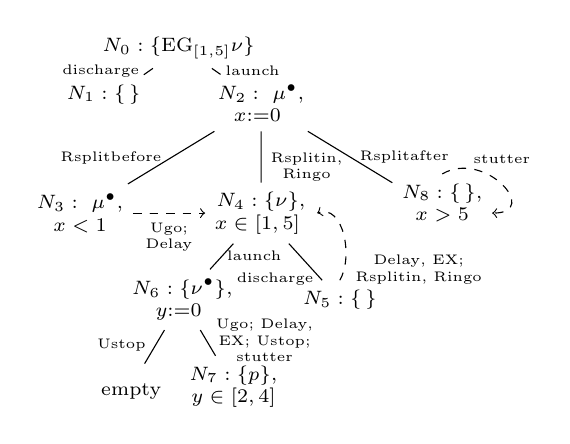
\begin{tikzpicture}[
  every node/.style={align=center, font=\scriptsize},
  level 1/.style={sibling distance=20mm, level distance=7mm},
  level 2/.style={sibling distance=23mm, level distance=14mm},
  level 3/.style={sibling distance=20mm, level distance=11mm},
  level 4/.style={sibling distance=13mm,level distance=11mm},
  edge from parent/.style={draw,-}
]
\node {$N_0:\{\mathrm{EG}_{[1,5]}\nu\}\ \ANDn$}
 child { node {$N_1:\{\,\}$\\ $\OPEN$}
   edge from parent node[left,font=\tiny,pos=.45]{\rl{discharge}} }
 child { node {$N_2:\ \mu^\bullet,$\\$x{:=}0\ \ANDn$}
   child { node (bef) {$N_3:\ \mu^\bullet,$\\$ x<1$}
    edge from parent node[left,font=\tiny,pos=.5]{\rl{Rsplitbefore}} }
   child { node (in) {$N_4:\{\nu\},$\\$ x\in[1,5]\ \ANDn$}
     child { node {$N_6:\{\nu^\bullet\},$\\$ y{:=}0\ \ORn$}
       child { node {$\CLOSED$\\ empty}
         edge from parent node[left,font=\tiny,pos=.45]{\rl{Ustop}} }
       child { node {$N_7:\{p\},$\\$ y\in[2,4]$}
         edge from parent node[right,font=\tiny,pos=.4]{\rl{Ugo}; \rl{Delay},\\ \rl{EX}; \rl{Ustop}; \\stutter} }
       edge from parent node[right,,xshift=-2pt,font=\tiny,pos=.45]{\rl{launch}} }
       child { node (disch) {$N_5:\{\,\}$}
       edge from parent node[left, yshift=-7pt,xshift=7pt,font=\tiny,pos=.45]{\rl{discharge}} }
     edge from parent node[right,font=\tiny,pos=.7]{\rl{Rsplitin},\\ \rl{Ringo}} }
   child { node (aft) {$N_8:\{\,\},$\\$ x>5$\\ $\OPEN$}
     edge from parent node[right,font=\tiny,pos=.5]{\rl{Rsplitafter}} }
   edge from parent node[right,font=\tiny,pos=.45]{\rl{launch}} };
\draw[->,dashed] (bef.east) to[out=0,in=180,looseness=.7]
  node[below,font=\tiny,pos=.5]{\rl{Ugo}; \\\rl{Delay}} (in.west);
\draw[->,dashed] (disch.north) to[out=60,in=20,looseness=1]
  node[right,yshift=-4pt,font=\tiny,pos=.25]{\rl{Delay}, \rl{EX};\\ \rl{Rsplitin}, \rl{Ringo} } (in.east);



\draw[->,dashed] (aft.north) to[out=30,in=0,looseness=2]
  node[above, yshift=4pt,font=\tiny]{stutter} (aft.east);
\end{tikzpicture}}
\subcaption{$\mathrm{EG}_{[1,5]}\tEU{\top}{p}{[2,4]}$.}\label{fig:ex-zeno}
\end{subfigure}
\caption{Two tableau runs. %$\ANDn$ marks an AND-node;$\ORn$ an OR-node. 
$\OPEN$ marks an open node, $\CLOSED$ a closed
one.}\label{fig:ex2}
\end{figure}

%\begin{example}%[A Zeno cycle that may be left]\label{ex:zeno}
Consider $\mathrm{EG}_{[1,5]}\,\nu$, where $\nu=\tEU{\top}{p}{[2,4]}$. Write $x$ for the clock of
the release, and $y$ for that of $\nu$. \ruleref{Cov} splits $N_0$ into a discharge child, which
carries no pursuit, and the launch $N_2$, where $x$ is reset. \ruleref{Rsplit} then partitions the zone,
conjunctively, into its three parts. At $N_3$, the \ruleref{Rsplitbefore} part, \ruleref{Delay} carries $x$ into  \kI. $N_8$, where $x>5$, drops $\mu^\bullet$ and leaves a goal-free node that
may delay indefinitely: a time-progressing loop, since no until needs to be fulfilled and $x$ is
extrapolated above $M$.
\noindent
$N_4$ represents the \ruleref{Rsplitin} part of \ruleref{Rsplit}, where $\nu$ is inserted into $\Gamma$ and so
demanded. \ruleref{Cov} applies, giving two conjunctive branches. The \ruleref{launch} child $N_6$
proves $\nu$. It carries $\nu^\bullet$ with $y$ reset; its \ruleref{Ustop} is empty there, the window
$[2,4]$ not yet open, so only \ruleref{Ugo} survives until a delay carries $y$ into $[2,4]$, where
\ruleref{Ustop} asserts $p$ and drops $\nu^\bullet$. The \ruleref{discharge} child $N_5$ drops $\nu$
from $\Gamma$ and carries $\mu^\bullet$ on; a delay and \ruleref{EX} revive the release, still inside
$[1,5]$, and its in-part demands $\nu$ once more. The search is back at $N_4$, closing a loop. That
loop is not time-progressing: $x$ is never reset, and the in-window zone holds it below $5$.
\noindent
Nonetheless, we can construct a successful marking  as $\mathcal M=\{N_0,\allowbreak N_1,\allowbreak N_2,\allowbreak N_3,\allowbreak N_4,\allowbreak N_5,\allowbreak N_6,\allowbreak N_7,\allowbreak N_8\}$. \ref{M2} holds because the only until pursuit is $\nu^\bullet$, active at $N_6$, and the path to
$N_7$ takes its \ruleref{Ustop} at a node whose zone meets $y\in[2,4]$. \ref{M1} holds because every node of
$\mathcal M$ reaches a time-progressing loop: the nodes carrying the release reach $N_8$ by delaying
until $x$ passes $5$, which lapses it, while $N_1$ and, once $\nu^\bullet$ is dropped, $N_7$ carry
no pursuit, so no deadline caps their delays and their stutter loops are time-progressing. So $\mathcal M$, as well as the tableau, are successful and
$\mathrm{EG}_{[1,5]}\,\nu$ is \SAT.

